\subsection{Balancing a segway}

\noindent Context: EL2222 Systems and Control in Practice
\noindent KTH Royal Institute of Technology, Stockholm, Sweden; 2015--2016 \\

\begin{problem}
Assume a two-wheeled motor-led contraption equipped with a
computing unit and an IMU. The goal is to balance the system in an upright
position using information from the gyro and the accelerometer.
\end{problem}


A basic solution consists of first integrating and fusing the angular velocity
and linear acceleration measurements to a Kalman filter that estimates the
system's angular error with respect to the vertical. The second step employs a
(in this case PID) controller that acts in a way that keeps this error at zero.
Figures \ref{fig:shellfie} and \ref{fig:shellfie_schem} show the real and
idealized ``shellfie" segway.

\noindent\makebox[\linewidth][c]{%
\begin{minipage}{\linewidth}
  \begin{minipage}{0.45\linewidth}
    \begin{figure}[H]\centering
      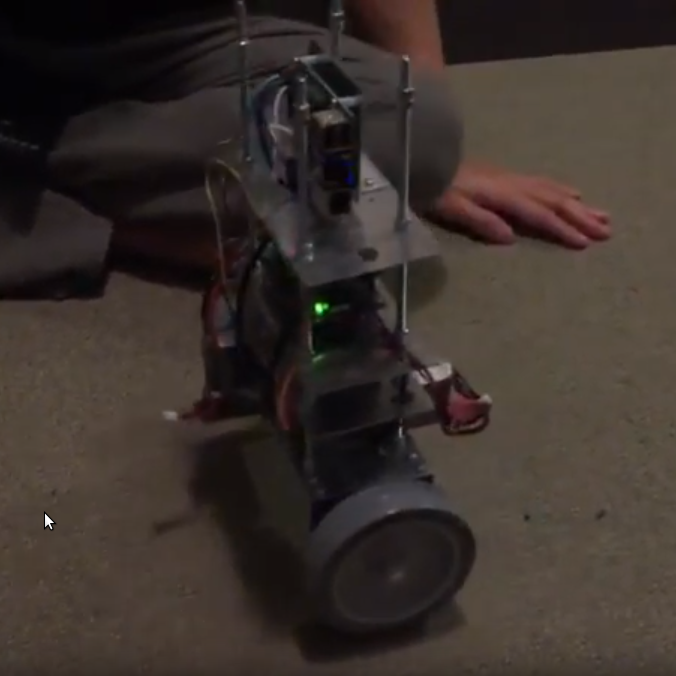
\includegraphics[scale=0.20]{images/shellfie.png}
      \caption{\small The custom-built ``shellfie" segway. Image courtesy of
               Jatesada Borsub}
      \label{fig:shellfie}
    \end{figure}
  \end{minipage}
  \hfill
  \begin{minipage}{0.45\linewidth}
    \begin{figure}[H]\centering
      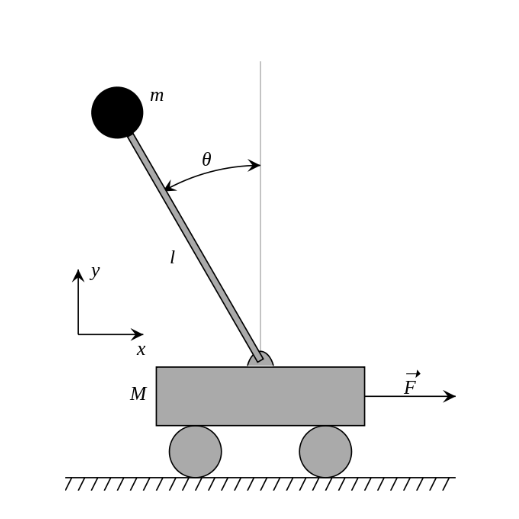
\includegraphics[scale=0.25]{images/shellfie_schem.png}
      \caption{\small The shellfie is in principle an inverted pendulum}
      \label{fig:shellfie_schem}
    \end{figure}
  \end{minipage}
\end{minipage}
}\\

\begin{itemize}
  \item Notions/resources/tools used: PID Control, Raspberry Pi, IMU, ROS, Linux, Python
\end{itemize}
